\chapter{Introduction} % Main chapter title


\label{Chapter1} % For referencing the chapter elsewhere, use \ref{Chapter1} 

\lhead{Chapter 1. \emph{Introduction}}
% \HRule \\[0cm]
Since recent years, web applications are becoming a popular alternative to traditional desktop applications.
% To access a web application, the end-user is only required to maintain a functioning web-browser, whereas the application vendor can deploy and update the application independent of end-users’ system configurations. 
During the evolution of a web application, it is repeatedly modified to add new functionality, fix bugs or adapt the GUI (Graphical User Interface) to improve the user experience. After such modifications, it is not uncommon to encounter side-effects manifested in the form of new bugs or re-emergence of old bugs. Such side effects usually occur as a result of changing system or component configurations, improper version control, applying incorrect or incomplete bug fixes etc. and can negatively affect the quality of the existing functionality. 

To ensure that after such modifications the application maintains its quality and still fulfills the existing specifications, regression tests are performed on the application under test (henceforth referred as AUT). Software developers typically re-run the existing test-suite along with a set of test inputs and test \textit{oracles} — mechanism to assess the test output, on a newly developed version to make sure that the code and functionality carried over from older version behaves as expected.

% Depending upon the development cycle, project size and available resources, regression tests can be performed at different abstraction levels, commonly as unit, integration and system testing. Unit tests are intended to test small pieces or modules of code, such as functions and classes, whereas integration tests are aimed to test the system as composition of different components. System level tests are performed at higher abstraction level similar to integration tests, however their goal is to check whether the software meets the functional specifications. 

Intuitively, in case of web applications the regression testing can be done at the GUI level, since majority of web applications’ functionality is accessed through this layer. In traditional sense, regression testing at GUI level abstracts away finer grained internal details by treating the AUT as a black-box. Such testing helps developers to identify the undesired  changes or an absence thereof in required functionality of the application.
% , since the GUI might have changed significantly while the underlying application has not. 

Dallmeier et al. \cite{webmate} presented the tool \texttt{webmate} for testing web 2.0 applications. To this date, \texttt{webmate} primarily functions as a cross-browser compatibility testing tool and supports different browsers and platforms. It can systematically explore the AUT by executing automated GUI tests and detect functional as well as GUI level differences in the AUT. 

As the application size increases, the possible combinations of inputs as well as GUI exploration paths also increase. Hence, GUI testing becomes more complicated as a typical GUI test involves multiple sequential operations since certain functionalities are only accessible through a series of GUI events.
% For example, to purchase an item in a typical e-commerce web application a user would need to perform sequential events such as login, add product to cart, fill payment details and finally checkout. This flow can vary depending on additional functionality such as purchasing pre-selected products, favourites etc. 
% As the possible number of paths and sequences increases, generating test inputs and applying test oracles becomes more difficult and costly. 
% Additionally, different browsers implement different technologies which might result in varied rendering of the GUI, making regression testing more complicated.

To reduce the costs incurred with manual testing, many developers choose to automate regression tests using Selenium\footnote{\url{http://www.seleniumhq.org/}} framework. The Selenium project provides the \texttt{webdriver} API to test dynamic web 2.0 applications. The API \textit{drives} i.e. controls the web browser in a manner that it emulates all possible user interactions with the application, such as clicks, form-inputs, file uploads etc. 
% Figure \ref{code1} illustrates 
As an example, to test the \textit{login} functionality of AUT as depicted in Figure \ref{fig:loginTest}, a \texttt{webdriver} based test \texttt{"loginTest"} would navigate to the homepage of AUT, fill the \textit{username} and \textit{password} fields and finally click the \textit{`Login'} button using the hyperlink-text ``Login'' as following (in Java):
\begin{small}
\texttt{driver.findElement(By.linkText("Login")).click()}
\end{small}
% \begin{minipage}{0.45\textwidth}
% % \begin{figure}
% 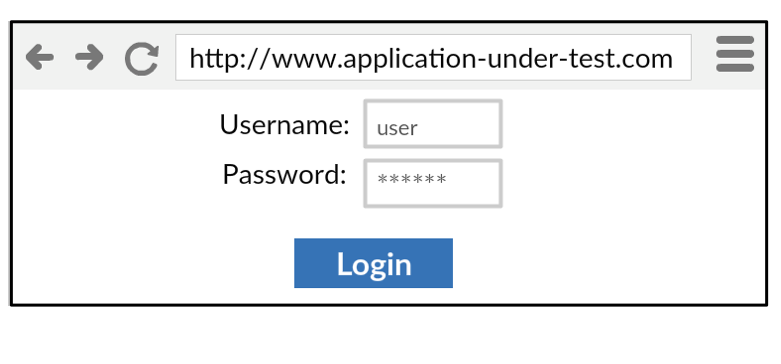
\includegraphics{./Figures/Login-button}
% \caption{Login}
% \label{fig:loginTest}
% % \end{figure}
% \end{minipage}%



% \begin{minipage}{0.5\textwidth}
% \begin{center}

% \begin{scriptsize}
% \lstset{
%   basicstyle=\ttfamily,
%   columns=fullflexible,
%   keepspaces=true,
% %   frame=none,
% }
% % \verb|basicstyle=\ttfamily, columns=fullflexible, keepspaces=true|
  
% \begin{lstlisting}[caption=Login test,label=code1]
% public void loginTest(){
% driver.get("http://www.application-under-test.com");
% driver.findElement(By.id("uname")).sendKeys("user");
% driver.findElement(By.id("pwd")).sendKeys("passwd");
% driver.findElement(By.linkText("Login")).click();
% }
% \end{lstlisting}
% \end{scriptsize} 
% \end{center}
% % \end{minipage}%

Compared to manual tests, Selenium tests can be run automatically and repeatedly. Typically, such tests can be combined with Continuous Integration tools to be run after the code changes are pushed to the version control repository. When AUT evolves from version $V_{0}$ to a newer version $V_{1}$, existing Selenium tests are executed on $V_{1}$. Ideally, if one or more tests executed successfully on $V_{0}$ fail to achieve the same result on $V_{1}$, the tests have found the possible software regressions in the AUT. In reality, this approach relies heavily on the quality and robustness of the existing tests. Robustness of Selenium tests implies their stability and effectiveness to achieve the same functional coverage across different versions of the AUT. 

However, as the web application continues to evolve, robustness of Selenium tests decreases over time. For newer versions, existing Selenium tests do not achieve the same functional coverage as they do for the version the tests are originally written for. Consider the aforementioned example of \texttt{loginTest} where the outcome of code changes results in changing the display text of \textit{`Login'} button's hyperlink to \textit{``Sign In''} in version $V_{1}$. When \texttt{loginTest} is re-run on $V_{1}$, it is unable to locate the \textit{`Login'} button since the hyperlink-text ``Login'' is changed to ``Sign in''. As a result, \texttt{loginTest} is broken and the desired functional coverage is not achieved unless this fragile test is repaired. 

To repair such fragile tests, developers need to invest time and efforts to analyze the functionality changes, identify test failures manually and maintain such test-suites. The reasons for decreasing robustness and failures of Selenium tests can include changed functionality, modified GUI element locators and changed structural markup, timing issues etc. If the AUT changes frequently, fragile tests need to be repaired repeatedly to cope with these changes which can be an expensive and time consuming task for developers. If Selenium tests are not robust and resilient enough as the AUT evolves, desired functional coverage is not achieved and regression testing is likely to be ineffective.
IF STRUCTURE BASED LOCATORS ARE USED, SLIGHT CHANGES IN PAGE STRUCTURE CAN MAKE THE TEST FRAGILE AND IF ATTRIBUTE BASED LOCATORS ARE USED THEN THEY WILL BE ROBUST AGAINST CHANGES 
% Robustness of Selenium tests can be defined in terms of their stability and effectiveness to achieve the same functional coverage across different versions of the AUT. 
% The reasons for decreasing robustness and failures of Selenium tests can include changed functionality, modified GUI element locators and changed structural markup, timing issues etc. 
% Such non-robust tests exhibiting decreased functional coverage are unsuitable for regression testing unless these tests are repaired. In order to modify such tests, developers need to invest time and efforts to analyze the undesired functionality changes, identify test failures manually and maintain such test-suites.

% In other words, if the Selenium tests are not robust enough, the regression testing is likely to be ineffective.

...........TILL HERE IS DONE .............

Considering the current state-of-the-art technologies to the extent of my knowledge, thus far there has been no research in the area of assessing the stability of Selenium tests across different versions of the web application. Currently there is no such technique to determine the robustness of Selenium tests over the version history of web applications to help developers write more robust tests and to understand the reasons behind brittleness of Selenium regression tests. 

% \begin{figure}
% \begin{subfigure}[b]{0.31\textwidth} 
% 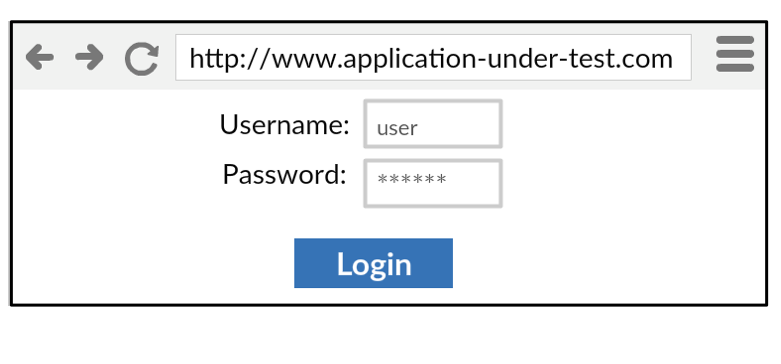
\includegraphics[width=7cm, height=3.2cm]{./Figures/Login-button}
% \caption{First subfigure}\label{fig:1a}
% \end{subfigure}
% \hspace*{\fill} % separation between the subfigures
% \begin{subfigure}{0.31\textwidth}
% 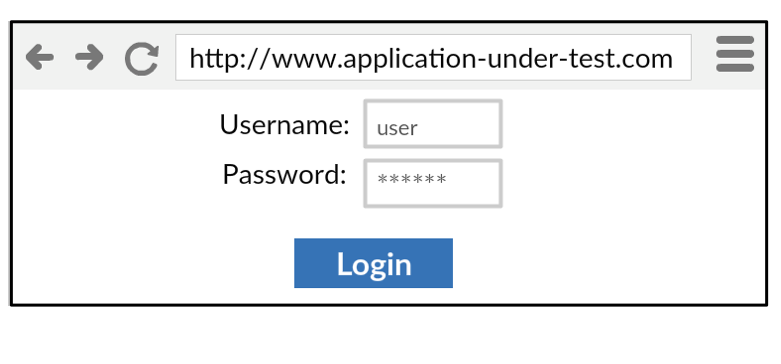
\includegraphics[width=7cm, height=3.2cm]{./Figures/Login-button}
% \caption{Second subfigure}\label{fig:1b}
% \end{subfigure}
% \caption{A figure that contains three subfigures}\label{fig:1}
% \end{figure}

% \subcaptionbox{The left subfigure with a long caption spanning several lines and some more text}%
%   [.4\linewidth]{\includegraphics[height=2cm]{example-image-a}}
%% THIS ONE WORKS !!!!!
\begin{figure}
\centering     %%% not \center
\subfigure[AUT version $V_{0}$]{\label{fig:a}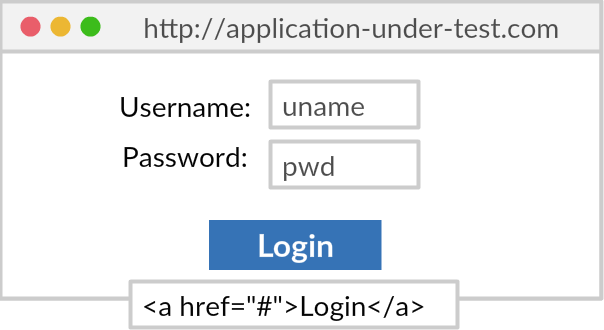
\includegraphics[width=5.6cm,height=2.8cm]{./Figures/newlogin}}
\vspace{-2mm}\subfigure[AUT version $V_{1}$]{\label{fig:b}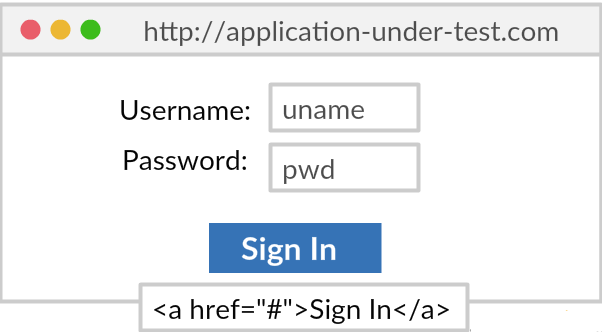
\includegraphics[width=5.6cm,height=2.8cm]{./Figures/newsignin}}
\caption{my caption}
\label{fig:loginTest}
\end{figure} 

% \begin{figure}
% 	\centering	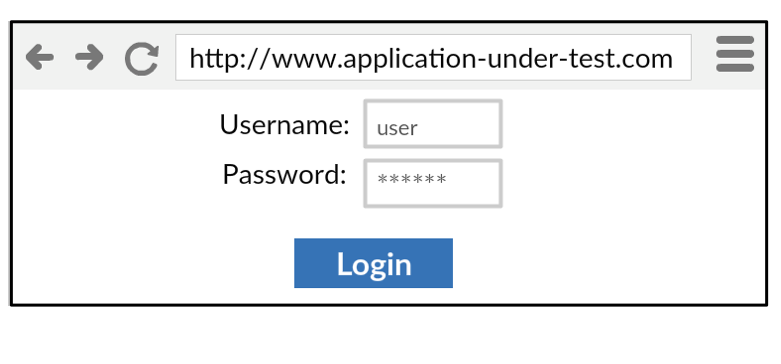
\includegraphics [width=7cm, height=3.2cm]{./Figures/Login-button}
% 	\caption{Login functionality of AUT}
% 	\label{fig:loginTest}
% \end{figure} 

The primary goal and scope of this thesis is to measure the robustness of Selenium regression test suites in comparison to different versions of web applications to determine whether there exists a correlation between the robustness of Selenium tests and changes in the AUT. To formally evaluate the approach and to investigate the reasons behind the varying robustness of Selenium tests \textit{robustness metric} has been defined (see Chapter X). Using the \textit{robustness metric} this thesis aims to assess the quality of open source Selenium tests and investigate the factors contributing towards the varying robustness of these tests.

 By providing developers a platform to evaluate their regression tests, this research aims to answer the following research questions:
{\bfseries RQ1} How to determine the robustness of Selenium tests?
{\bfseries RQ2} Is the change in robustness correlated to the changes of application’s structural elements?
{\bfseries RQ4} Do tests with shorter execution traces tend to be more robust than tests with relatively longer traces?
{\bfseries RQ5} Does same test input result in different GUI states of the AUT for different versions (\textit{reachability problem})?
{\bfseries RQ6} Can the robustness analysis improve or assist current regression testing practices?
{\bfseries RQ7} Reasons of failure behind test cases?
{\bfseries RQ8} Size and complexity of test suite?

The Figure XXX depicts the setup model required for the robustness analysis. The first step is to select suitable testing candidates for the research and extract Selenium tests-suites for each candidate from their test repositories. The approach is to test setup and deploy different versions of test candidates AUT and run automated Selenium regression tests on them.
In the next step, Selenium tests are leveraged to capture the application behavior as trace level and GUI level models, which are then compared with the output logs of Selenium tests.ADD MORE INFO.
***Add what makes a test robust, how we detect the robustness, whats the assumption (equal actions) - how a test can pass and still not be robust
In order to formally assess the changes in robustness of the tests, robustness metric is defined as detailed in section XXX. Using the robustness metric as well as the trace level and GUI level differences, robustness of Selenium tests analyzed.
***If the presented model detects failures etc
\begin{figure}
% [htbp]
	\centering	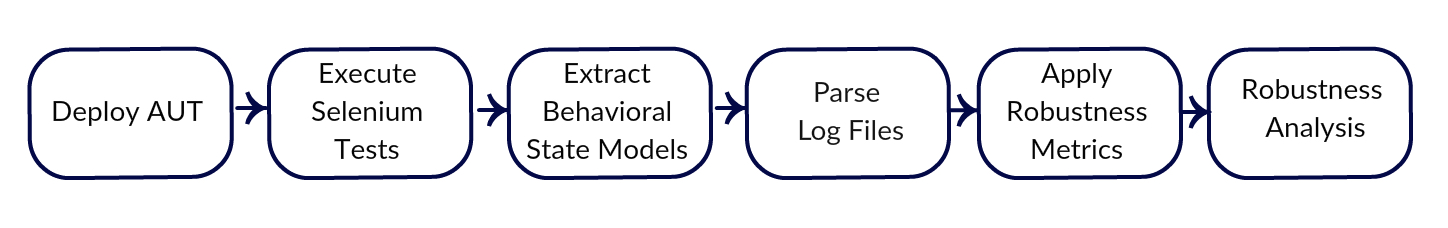
\includegraphics[width=\textwidth]{./Figures/thesisoverviewsmall.jpg}
%     [width=5cm, height=3cm]
% 		\rule{35em}{0.5pt}
	\caption{Setup required for the robustness analysis}
	\label{fig:thesisoverview}
\end{figure} 

…..ORGANIZATION….
Introduction 4 pages
Chapter 2 discusses the background automated GUI testing, WebMate, Statistical analysis background, 4 pages
Chapter 3 discusses Factors affecting Robustness of Selenium tests, sample errors, fluentwaits, stale element exception etc. 6 pages
Chapter 4 discusses Approach and Evaluation : 20 pages
Approach: Candidate selection, deployment, modifying selenium tests to fit to remotewebdriver, using sessionIDs to track, explaining how the entire grid works, extraction of state-models, comparison of GUI sequences, major minor versions,
Evaluation: Experimental setup, test results, robustness metrics calculation, graphs, results
For evaluating the approach and answer the research questions, the idea was to assess publicly available Selenium tests, in order to eliminate the possible bias introduced by writing one’s own Selenium tests as such are written from a single person’s design approach. In the same spirit, the presented model is tested on six different open source projects, from different domains as follows: (MAKE A TABLE)
Name: website:domain
Jenkins LTS, Jenkins, Mozilla Addons, Mozilla Marketplace, mozilla.org, moodle
All of these projects feature open source Selenium tests written in Java as well as Python and the presented approach leverages these tests for the purpose of this research. (Add connectors)
Chapter 5 discusses threats to validity 2 pages
Chapter 6 discusses conclusion and future work 2 pages
 

